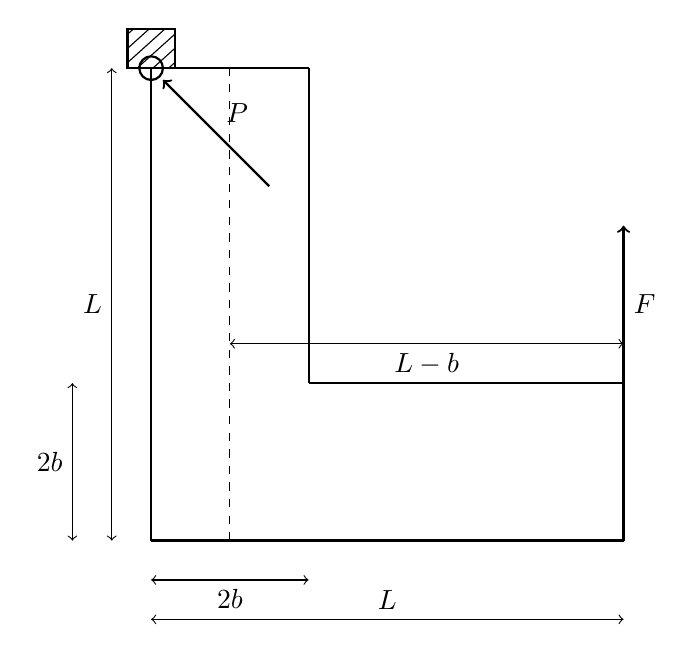
\begin{tikzpicture}

    % Draw the L-shaped structure
    \draw[thick] (0,0) -- (0,6); % vertical part
    \draw[thick] (0,0) -- (6,0); % top horizontal part
    \draw[thick] (0,6) -- (2,6); % downward part
    \draw[thick] (2,2) -- (6,2); % bottom horizontal part
    \draw[thick] (2,2) -- (2,6); % vertical part
	\draw[thick] (6,0) -- (6,2);

    % Draw the wall (left)
  \begin{scope}
    % Clip to the shape
    \clip (-0.3,6) rectangle (0.3,6.5);
    % Draw diagonal lines
    \foreach \x in {-6,-5.8,...,6} { % Adjust spacing by modifying the range
        \draw[thin] (\x,5.8) -- (\x+1,6.7); % Adjust the angle and range as needed
    }
\end{scope}

% Outline the shape
\draw[thick] (-0.3,6.5) -- (0.3,6.5) -- (0.3,6) -- (-0.3,6) -- cycle;

    % Draw hinge circle at the corner
    \draw[thick] (0,6) circle (0.15);

    % Forces
    \draw[thick,->] (6,2) -- (6,4) node[midway, right] {$F$}; % Force F
    \draw[thick,<-] (0.15,5.85) -- (1.5,4.5) node[midway, above right] {$P$}; % Force P

    % Dimensions
    \draw[<->] (-0.5,0) -- (-0.5,6) node[midway, left] {$L$}; % Left dimension L
    \draw[<->] (0,-0.5) -- (2,-0.5) node[midway, below] {$2b$}; % Bottom dimension 2b
    \draw[<->] (1,2.5) -- (6,2.5) node[midway, below] {$L-b$}; % Middle dimension L-b
    \draw[<->] (0,-1) -- (6,-1) node[midway, above] {$L$}; % Right dimension L
	\draw[<->] (-1,0) -- (-1,2) node[midway, left] {$2b$};
    
    % Dashed line (center axis for the square at the bottom)
    \draw[dashed] (1,0) -- (1,6);

   \end{tikzpicture}
